% document style header
\documentclass[a4paper, 12pt]{config/homework}

% import default packages
\usepackage{config/defpackages}
% import custom math commands
\usepackage{config/domath}
\usepackage{pdfpages}

% end preamble
\begin{document}

% document title
\noindent
\begin{tabularx}{\textwidth}{>{\centering\arraybackslash}X>{\centering\arraybackslash}X>{\centering\arraybackslash}X}
Calvin Sprouse & PHYS489 Goal 4A & 2024 February 21\\
\midrule
\end{tabularx}

% homework problems begin
% 4A Oral scientific communication
% Select an artifact associated with an oral presentation in which you communicated scientific ideas and write a reflection statement describing ways in which your presentation demonstrated effective oral scientific communication. In preparing your reflection, consider that effective oral presentation skills include “knowing your audience” and adapting your explanations to be accessible to non-experts; exercising judgment to determine which content to include within a limited time allocation; framing the “big picture”; and delivering the presentation in an organized and clear manner. Examples of oral scientific communication might include presentations at SOURCE or another conference (posters or talks), a formal presentation in a physics class, a planetarium show or other public presentation.

Below is an oral presentation I gave with my research group for SOURCE 2023. The primary goal of this presentation was to tell the story of our research in such a way that a broad undergraduate audience could understand. To create this presentation we started with a poster that we had brought to the Biophysical Society Meeting 2023 as it would contain nearly all the information we felt was relevant to the project. The only thing this poster was missing was adequate background for a non-professional audience. In adding that background some finer details about the model were cut. We made this decision with the belief that our audience would be more interested in contextualizing results in terms of the biological system. To deliver this broad background effectively our presentation is mostly image and video based using cartoon models to illustrate behavior leading up to clearly labeled plots to indicate results. This is the fourth official revision with each one having significant changes from its predecessor. Not to mention the many practice attempts and script changes. We gave this presentation at SOURCE 2023 in front of physics majors, chemistry majors, and biology majors which matched our expectations for a broad audience. The presentation went very well and I am very fortunate for having that experience of professional public speaking.

% add pdf pages
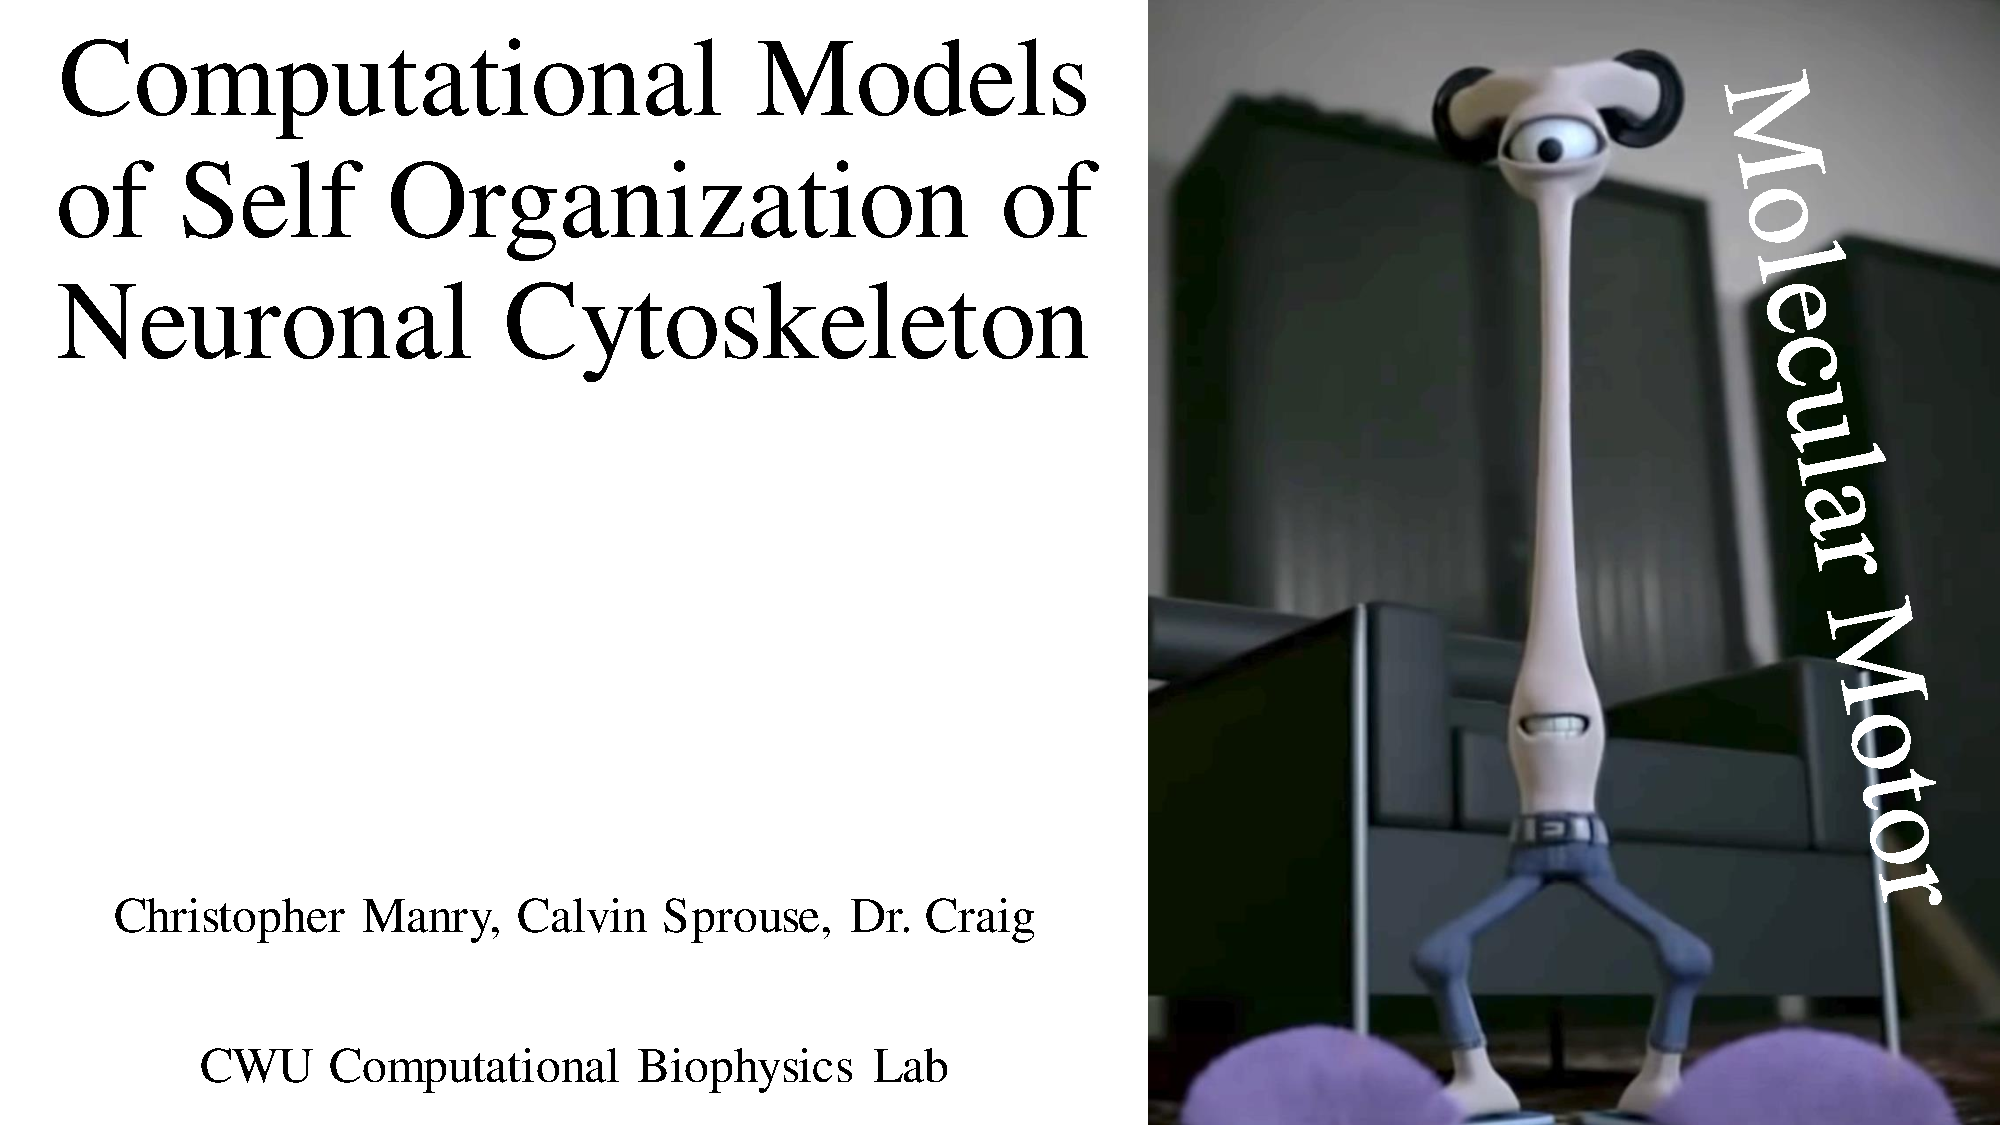
\includepdf[pages=-, angle=90]{source2023_presentation.pdf}

\end{document}
